\documentclass[11pt,a4paper]{article}
\usepackage[utf8]{inputenc}
\usepackage[T1]{fontenc}
 
\usepackage{lmodern}
\usepackage[french]{babel}


\usepackage[margin=1in]{geometry} 
\usepackage[parfill]{parskip}

\usepackage{amsfonts}
\usepackage{amssymb}
\usepackage{amsmath}
% add system ( emphased equation )
\usepackage{empheq}
%mfrac
\usepackage{nccmath}
\usepackage{xcolor}
\usepackage{float}
\usepackage{graphicx}
\usepackage{hyperref}

\usepackage{caption}
\usepackage{subcaption}
%\usepackage{csquotes}
\usepackage{enumitem}
\usepackage{multirow}
\usepackage{longtable}
%\usepackage[style=ieee]{biblatex}
\usepackage{todonotes}
\usepackage{pdfpages}
\setlist[itemize,1]{label=$\circ$}
\setlist[enumerate,1]{label=(\alph*), ref=\thesection(\alph*)}
\setlist[enumerate,2]{label=\roman*., ref=\thesection(\alph{enumi}).\roman*}
\newcommand{\magikpdf}[2]{
        \includepdf[pages=-,width=0.9\paperwidth,pages={1},clip,
pagecommand={#1}]{#2} % wierd wizard stuff
}
\usepackage{lipsum}
\usepackage{listings}
\newcommand{\dd}{d_1}
\newcommand{\dt}{d_T}
\newcommand{\da}{d_A}
\newcommand{\blank}{\mathrel{\underline{\hspace{2em}}}}
\newcommand{\Ma}{M_A}
\newcommand{\Mt}{M_T}
\newcommand{\Na}{N_A}
\newcommand{\Nt}{N_T}
\newcommand{\ddd}{d_2}
\newcommand{\Fr}{F_r}
\newcommand{\Ft}{F_t}
\newcommand{\Fa}{F_a}


\DeclareMathOperator{\Var}{Var}

\newcommand{\cotan}{\mathrm{cotan}}

\begin{document}
\begin{titlepage}
\begin{minipage}{0.5\textwidth}
\begin{flushleft} 

\includegraphics[height=2.3cm]{template/Im1.PNG}
\end{flushleft}
\end{minipage}
\begin{minipage}{0.5\textwidth}
\begin{flushright} 

\includegraphics[height=1.9cm]{template/Im2.PNG} 
\end{flushright}
\end{minipage} \\ [3cm]

\begin{center}
\textsc{\LARGE Université de Liège}\\[0.5cm]
\textsc{\Large Faculté des Sciences Appliquées}\\[3.0 cm]
\noindent\rule{\textwidth}{0.4mm} \\[.7cm]
\textsc{\LARGE SYST0002 }\\[0.7cm]
\textsc{\LARGE  Introduction aux signaux et systèmes}\\[0.7cm]
\textsc{\LARGE  Projet}\\[0.7cm]
%\textsc{\LARGE\textit{ }}\\[0.5cm]

\end{center}
\noindent\rule{\textwidth}{0.4mm}
\vspace*{10mm}

    \textsc{\large DELBARRE} \large Loïc (S215072) \\[1mm]
    \textsc{\large JACQUEMIN} \large Justin (S224395) \\
\begin{center}
\vfill
{\large Bachelier Ingénieur Civil
\\[.3cm]
Année Académique 2024-2025}
\end{center}
\end{titlepage}
\setcounter{tocdepth}{3}
\pagebreak
%\listoffigures
%\newpage
\tableofcontents
\newpage

%%%%%%%%%%%%%%%%%%%%%%%%%%%%%%%%%%%%%%%%%%%%%%%%%%%%%%%%%%%%%%%%%%%%%%%

\section{Part 1: modèle d'état, linéarisation et simulations}
\subsection{linéarité du modèle dynamique}
Le modèle considéré est non-linéaire.
En effet pour qu'un système soit linéaire , il faut que celui ci puisse s'écrire de la forme :
$$ a_n (x) y^{(n)}+ ..$$
Or à cause du terme $\sin(\alpha(\delta(t)+\theta(t))$ , celui ci fair apparaitre de la non-linéarité pour $\theta$
\subsection{paramètre du système}
\begin{itemize}
    \item entrées : $\delta(t)$
    Le delta est associé à l'orientation des roue par rapport à l'axe du véhicule en fonction du temps.Son image appartient à l'intervale $[-\dfrac{\pi}{2},\dfrac{\pi}{2}]$
    \item sorties : $s(t)$
    La sortie est position selon l'axe vetical
    \item variables d'états : $y(t),\theta(t)$
    Y représente également l'évolution temporelle de la position selon l'axe vertical.Il n'y a pas de contrainte dans l'énoncé , on peut donc supposer que son domaine de définition ainsi que son image appartiennent à $\mathbb{R}$
    $\theta$ quant'à lui représente l'évolution temporelle de l'orientation du véhicule dans l'espace.Vu qu'il s'agit d'un angle , on peut raisonablement restreindre son image à l'intervale $[ 0,2\pi]$
    \item constantes: a est la distance entre l'axe arrière et le centre de masse du véhicule.Et b , la distance entre l'axe des roues avant et celui des roues arrière.$v_0$ représente la vitesse du centre de masse.
\end{itemize}
Pour tout les signaux mentionnés , nous supposeront que $t \in \mathbb{R}^+$
\subsection{simulation du système}
\subsubsection{cas d'un mouvement sans tourner}
\begin{figure}[!h]
    \centering
    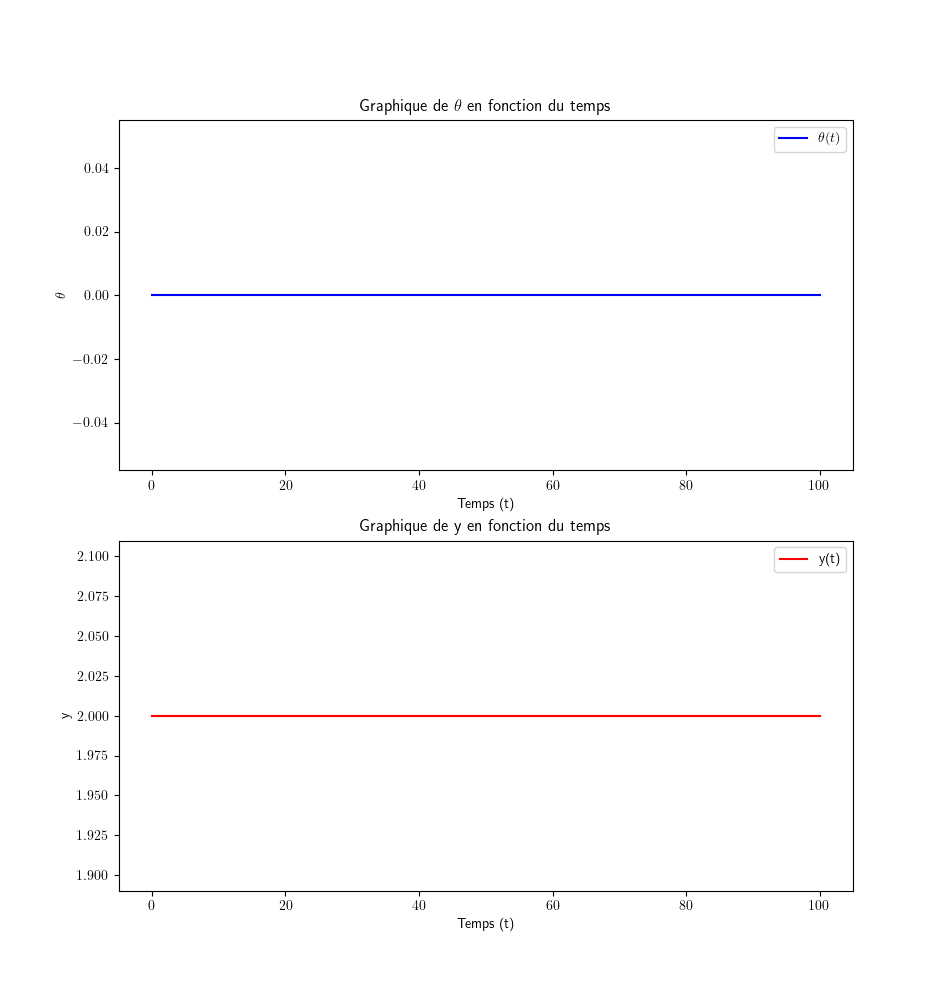
\includegraphics[width=0.5\linewidth]{Q3_flat.png}
\end{figure}
\newpage
\subsubsection{cas d'une mouvement dont les roues oscillent sinusoidalement}
\begin{figure}[!h]
    \centering
    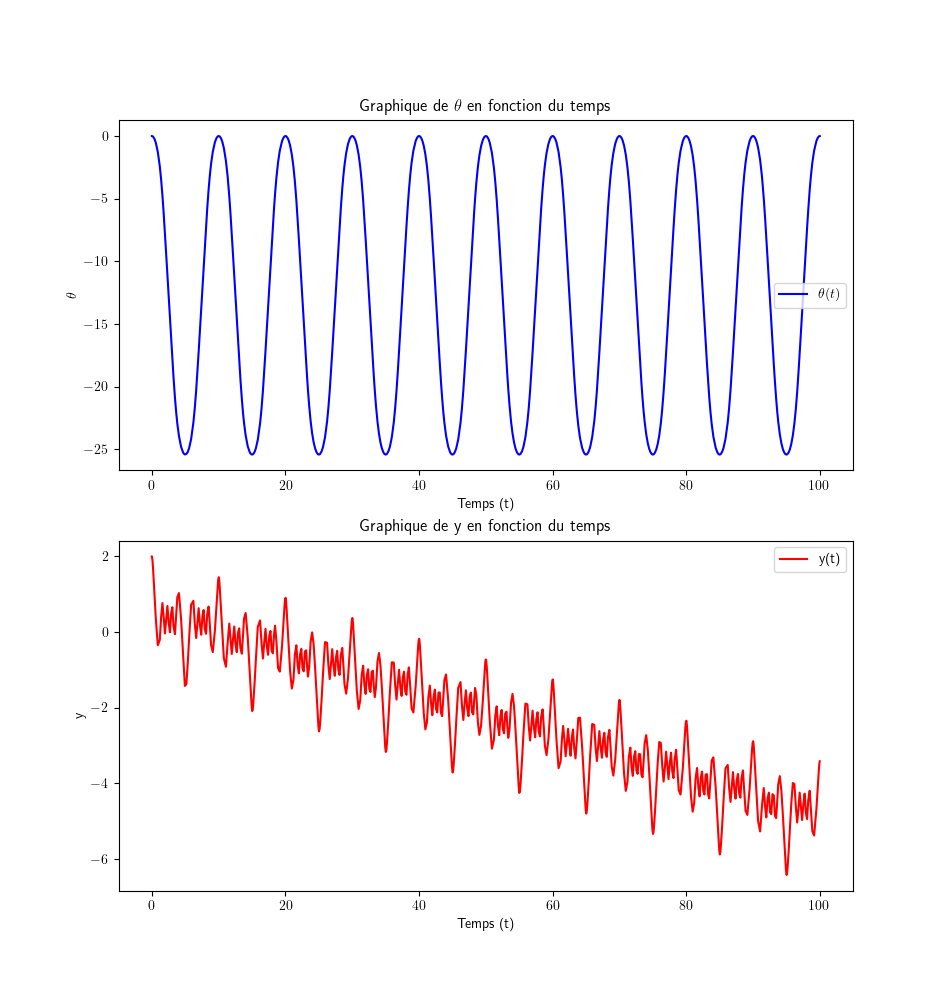
\includegraphics[width=0.5\linewidth]{Q3.png}
\end{figure}
\subsection{Points d'équilibre du système}
Dans le cadre de ce rapport , la notation $\dot y$ correspond à $\dfrac{d y}{dt}$.
Afin de trouver les points d'équilibre du système de manière analytique il suffit de trouver :
\begin{equation}
    \begin{cases}
      \dot y=0\\
      \dot \theta=0= \dfrac{v_0 sin \alpha(\delta (t) )}{a}
    \end{cases}
\end{equation}
On trouve donc par la deuxième équation que 
$$\delta(t) = k\pi \quad \text{avec} \quad k \in \mathbb{Z}$$

De la, en découle via la première équation que 
$$\theta(t)=k\pi \quad \text{avec} \quad k \in \mathbb{Z}$$
On trouve donc dans le système deux point d'équilibre au vu des domaines et des images.On a donc $(\delta;\theta)=(0;0)$ ou bien $(\delta;\theta)=(0;\pi)$ 
\subsection{Matrice d'état A,B,C,D}
Afin de trouver les matrice d'état du système il faut se baser sur la méthode des dérivées.
On identifie aisément que :
\begin{equation}
    \begin{cases}
     f= v_0 \sin(\alpha(\delta(t)+\theta(t)) \\
     g= \dfrac{v_0 sin(\alpha(\delta(t))}{a} 
    \end{cases} 
\end{equation}
Les matrices sont donc calculé via les dérivées au point d'équilibre du système:
\begin{equation}
\begin{cases}
    A= \begin{pmatrix}
        0 & \pm v_0 \\
        0 & 0
    \end{pmatrix} \\
        B= \begin{pmatrix}
        \dfrac{\pm v_0 a}{b}  \\
        \dfrac{\pm v_0}{b}  
    \end{pmatrix} \\
            C= \begin{pmatrix}
            1 & 0 
    \end{pmatrix}\\
            D= \begin{pmatrix}
        0  
    \end{pmatrix}
\end{cases}
\end{equation}
Ce qui peut s'écrire sous forme matricielle : 
\[
\frac{d}{dt}
\begin{pmatrix}
    y(t) \\
    \theta(t)
\end{pmatrix}
=
\begin{bmatrix}
    0 & \pm v_0 \\
    0 & 0
\end{bmatrix}
\begin{pmatrix}
    y(t) \\
    \theta(t)
\end{pmatrix}
+
\begin{bmatrix}
    \pm v_0 \frac{a}{b} \\
    \frac{\pm v_0}{b}
\end{bmatrix}
\delta(t).
\]

    \subsection{nature des points d'équilibre}
La matrice Jacobienne pour les points d'équilibre est déterminé via
$ det(A-\lambda \mathbb{I})=0 $.On obtient donc que les valeur permisent pour lambda sont nulles.On ne peux donc rien conclure concernant la stabilité du système.
\subsection{simulation au point d'équilibre}



\begin{figure}[!h]
    \centering
    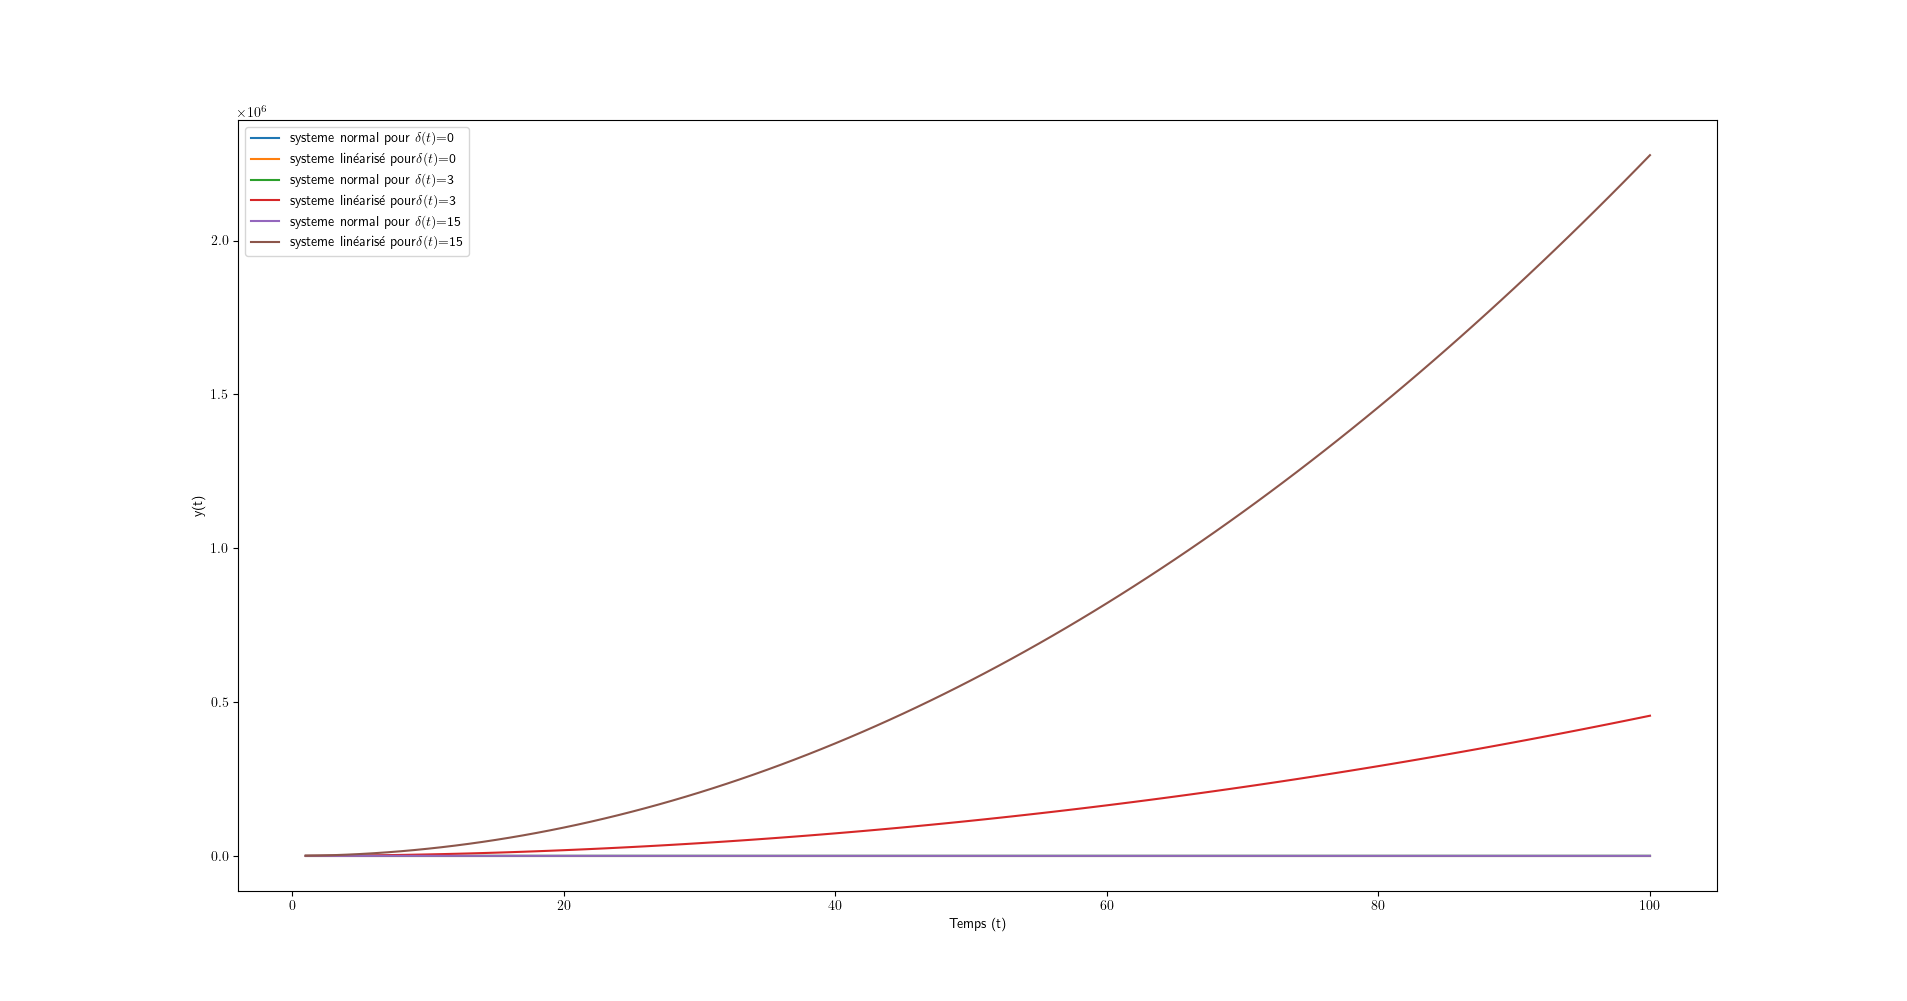
\includegraphics[width=0.5\linewidth]{Q7.png}
\end{figure}
On peut constater que les fonctions non linéaire ont le même résultat que celle du modèle ABCD.Vu que $\delta$ étant constant , la valeur de $\dot \theta$ n'est pas modifié au fur et a mesure du temps et donc pour $\theta>0 $ on appercois une augmentation de y(t) constante qui est représenté sur la courbe par la courbure exponentielle.










\subsection{trajectoire gaussienne}
Actuellement nous avons essayé plusieurs méthode sans parvernir à trouver une solution 
\subsubsection{résolution analytique}
On peut se pencher sur le système linéarisé , et deviner par identification quels facteurs permetteraient d'avoir le nombre et la valeurs des coefficient de nos gaussienne.
en réinjectant la deuxième équation linéarisé dans la première on se réduit à l'équation différentielle suivante:
$$\dot y = v_0 \dfrac ab  \delta + \dfrac{v_0} b \dot \delta $$
La solution recherché est 
$$y= \dfrac{25}{\sqrt{2 \pi \sigma^2}} exp(\dfrac{-(t-\mu)^2}{2\sigma^2})$$
Sa dérivée par rapport au temps est donc
$$\frac{dy}{dt} = -\dfrac{25(t-\mu)}{\sqrt{2 \pi \sigma^2} \sigma^2} \exp\left(\dfrac{-(t-\mu)^2}{2\sigma^2}\right)$$
l'équation différentielle se réecrit donc :
$$-\dfrac{25(t-\mu)}{\sqrt{2 \pi \sigma^2} \sigma^2} \exp\left(\dfrac{-(t-\mu)^2}{2\sigma^2}\right) = v_0 \dfrac{a}{b} \sum^n_{i=0} \left( \dfrac{A_i}{\sqrt{2\pi\sigma_i^2}} \exp \left(\dfrac{-(t-\mu_i)^2}{2\sigma_i^2}\right) \right)+\dfrac{v_0}{b}\sum^n_{i=0} \left(-\dfrac{A_i(t-\mu_i)}{\sqrt{2 \pi \sigma_i^2} \sigma_i^2} \exp\left(\dfrac{-(t-\mu_i)^2}{2\sigma_i^2}\right)\right)$$
Si l'on considère n=1
on obtient 
$$-\dfrac{25(t-\mu)}{\sqrt{2 \pi \sigma^2} \sigma^2} \exp\left(\dfrac{-(t-\mu)^2}{2\sigma^2}\right) = v_0 \dfrac{a}{b} \left( \dfrac{A_0}{\sqrt{2 \pi \sigma_0^2}} \exp \left( \dfrac{-(t-\mu_0)^2}{2\sigma_0^2} \right) \right) + \dfrac{v_0}{b} \left( -\dfrac{A_0(t-\mu_0)}{\sqrt{2 \pi \sigma_0^2} \sigma_0^2} \exp \left( \dfrac{-(t-\mu_0)^2}{2\sigma_0^2} \right) \right)
$$
Le reste du développement est encore à faire 
Mais il semble montrer qu'il y ait moyen d'utiliser une seule Gaussienne .
\subsubsection{résolution numérique}
On peut supposer le problème comme étant la minimization d'une fonction prennant en argument une matrice colone de taille 3n représentant les différents paramètre associé au différentes Gaussiennes et retournant le Mean square error comparé a la trajectoire attendue .
Actuellement nous avons fait tourner sans succès notre minimization pour des tailles de matrice allant jusqu'a 15 élément.
\subsubsection{dernière piste non exploré}
Une dernière piste non exploré , serait de passer en domaine fréquentiel au vu de la fonction demdandé.
\section{State-feedback controller, simulations et analyse de Fourier}
\subsection{}
\subsection{calcul des matrices d'état du système global}
En remplacant l'équation du controller dans celle du Plant , on obtient:
\begin{equation}
\begin{cases}
\dot x= (A-KB)x+BK_rr \\
s= (C-KD)x+DK_rr
\end{cases}
\end{equation}
Par identification,on remarque donc que : \\
\begin{equation}
\begin{cases}

\tilde{A} = A-KB \\
\tilde{B} = K_rB \\
\tilde{C} = C-KD \\
\tilde{D} = K_rD \\

\end{cases}
\end{equation}

\end{document}
